\documentclass[11pt]{article}

\usepackage[margin=1in]{geometry}
\usepackage{graphicx}
\usepackage{array}
\usepackage{hyperref}
\usepackage{enumitem}
\usepackage{booktabs}
\usepackage{caption}
\usepackage{amsmath}
\usepackage{titlesec}
\usepackage{float}
\titleformat{\section}{\large\bfseries}{\thesection.}{1em}{}

\begin{document}

\begin{center}
    \Large \textbf{Sri Sivasubramaniya Nadar College of Engineering, Chennai} \\
    \large (An Autonomous Institution affiliated to Anna University) \\
    \vspace{0.3cm}
\end{center}

\begin{table}[H]
\renewcommand{\arraystretch}{1.4}
\resizebox{\textwidth}{!}{%
\begin{tabular}{|l|l|l|l|}
\hline
Degree \& Branch & B.E. Computer Science \& Engineering & Semester & VI \\ \hline
Subject Code \& Name & \multicolumn{3}{l|}{UCS2612 – Machine Learning Algorithms Laboratory} \\ \hline
Academic Year & 2025–2026 (Even) & Batch & 2023–2027 \\ \hline
Name & Munish Madhav M & Register No. & 3122235001086 \\ \hline
Due Date & \multicolumn{3}{l|}{07.03.2026} \\ \hline
\end{tabular}}
\end{table}


\begin{center}
    \textbf{\Large Experiment 6}
\end{center}

\begin{center}
    \textbf{Decision Tree and Random Forest: A Comparative Classification Study}
\end{center}

%--------------------------------------------------

\section*{Objective}

To implement and compare the performance of:
\begin{itemize}
    \item \textbf{Model A:} Decision Tree classifier
    \item \textbf{Model B:} Random Forest ensemble model (extension of Decision Trees)
\end{itemize}

Students must study the impact of hyperparameters on overfitting and generalization, perform hyperparameter tuning using 5-Fold Cross-Validation, and compare the performance between single-tree and ensemble-based models.

%--------------------------------------------------

\section*{Dataset}
\textbf{Wisconsin Diagnostic Breast Cancer Dataset}

\begin{itemize}
    \item Total samples: 569
    \item Features: 30 numerical attributes
    \item Target classes: Malignant (M) and Benign (B)
\end{itemize}

\textbf{Dataset Link:}  
\href{https://archive.ics.uci.edu/dataset/17/breast+cancer+wisconsin+diagnostic}{https://archive.ics.uci.edu}

%--------------------------------------------------

\section*{Theory}

\subsection*{Decision Tree Classifier}
A Decision Tree is a supervised learning model that recursively splits the feature space using impurity measures to form decision rules.

\textbf{Key Concepts:}
\begin{itemize}
    \item Gini Index and Entropy
    \item Tree depth and node splitting
    \item Overfitting in deep trees
\end{itemize}

\textbf{Limitation:}  
Decision Trees are prone to high variance and overfitting.

\subsection*{Random Forest Classifier}
Random Forest is an ensemble learning technique that combines multiple decision trees trained on bootstrapped samples.

\textbf{Key Ideas:}
\begin{itemize}
    \item Bootstrap aggregation (bagging)
    \item Random feature selection
    \item Majority voting
\end{itemize}

\textbf{Advantage:}  
Reduces variance and improves generalization compared to a single Decision Tree.

%--------------------------------------------------
\section*{Implementation Summary}

The dataset was loaded and the target labels were encoded. Exploratory Data Analysis (EDA) was performed to observe class distribution and feature correlations. The data was then split into an 80--20 training and testing set.

Both Decision Tree and Random Forest classifiers were trained, and optimal hyperparameters were selected using 5-Fold Cross-Validation (GridSearchCV). Finally, the models were evaluated and compared using multiple performance metrics.


%--------------------------------------------------
%--------------------------------------------------

\section*{Hyperparameter Tuning Results}

\subsection*{Decision Tree Cross-Fold Results}

\begin{table}[H]
\centering
\caption{Decision Tree Hyperparameter Evaluation (Top 5 Results)}
\renewcommand{\arraystretch}{1.3}
\begin{tabular}{cccc}
\toprule
Criterion & Max Depth & Avg CV Accuracy (\%) & Avg CV F1 Score \\
\midrule
entropy & 3 & 94.29 & 92.32 \\
entropy & 5 & 94.29 & 92.06 \\
entropy & 5 & 94.29 & 92.06 \\
entropy & 10 & 94.29 & 92.06 \\
entropy & None & 94.29 & 92.06 \\
\bottomrule
\end{tabular}
\end{table}

\subsection*{Random Forest Cross-Fold Results}

\begin{table}[H]
\centering
\caption{Random Forest Hyperparameter Evaluation using 5-Fold Cross-Validation}
\renewcommand{\arraystretch}{1.3}
\begin{tabular}{ccccc}
\toprule
n\_estimators & Max Depth & Max Features & Avg CV Accuracy (\%) & Avg CV F1 Score \\
\midrule
50 & 10 & sqrt & 96.48 & 95.15 \\
50 & 20 & sqrt & 96.48 & 95.15 \\
50 & None & sqrt & 96.48 & 95.15 \\
200 & None & sqrt & 96.26 & 94.88 \\
100 & None & log2 & 96.26 & 94.92 \\
\bottomrule
\end{tabular}
\end{table}

%--------------------------------------------------

\section*{5-Fold Cross-Validation Performance Comparison}

\begin{table}[H]
\centering
\caption{5-Fold Cross-Validation Accuracy Comparison}
\renewcommand{\arraystretch}{1.3}
\begin{tabular}{lcccccc}
\toprule
Model & Fold 1 & Fold 2 & Fold 3 & Fold 4 & Fold 5 & Average \\
\midrule
Decision Tree & 0.9780 & 0.9121 & 0.9451 & 0.9451 & 0.9341 & 0.9429 \\
Random Forest & 0.9780 & 0.9560 & 0.9670 & 0.9780 & 0.9451 & 0.9648 \\
\bottomrule
\end{tabular}
\end{table}

%--------------------------------------------------
\section*{Hyperparameter Analysis}

In this experiment, optimal model configurations were identified using 5-Fold Cross-Validation. The hyperparameter search space was designed to balance the bias-variance tradeoff, with a particular focus on mitigating the overfitting tendencies of Decision Trees.

\subsection*{1. Decision Tree Parameter Analysis}

The Decision Tree tuning focused on parameters that control node splitting and tree growth:

\begin{itemize}
    \item \textbf{Criterion (gini vs.\ entropy):} This parameter determines the function used to measure the quality of a split. While Gini impurity is computationally faster, Entropy can sometimes produce more balanced trees by maximizing information gain. The observed differences in performance were minimal for this dataset.
    
    \item \textbf{Max Depth (\texttt{max\_depth}):} This is the most critical hyperparameter for controlling overfitting. Allowing unrestricted depth (None) often leads to memorization of training data, reducing generalization. Limiting the depth (e.g., 3 or 5) acts as pre-pruning and helps capture only the most significant patterns.
    
    \item \textbf{Minimum Samples (\texttt{min\_samples\_split}, \texttt{min\_samples\_leaf}):} Increasing these values enforces stricter conditions for node splitting and leaf formation. This acts as regularization, resulting in smoother decision boundaries and reduced variance.
\end{itemize}

\subsection*{2. Random Forest Parameter Analysis}

The Random Forest tuning focused on ensemble-level parameters and constraints on individual trees:

\begin{itemize}
    \item \textbf{Number of Estimators (\texttt{n\_estimators}):} This defines the number of trees in the forest. Increasing this value improves stability and reduces variance, but performance tends to plateau beyond a certain point (typically around 100--200 trees).
    
    \item \textbf{Max Features (\texttt{max\_features}):} Limiting the number of features considered at each split (e.g., \texttt{sqrt}, \texttt{log2}) enforces randomness among trees. This de-correlation is key to reducing variance in the ensemble.
    
    \item \textbf{Bootstrap:} Enabling bootstrapping ensures that each tree is trained on a randomly sampled subset of the dataset with replacement. This increases robustness to noise and outliers.
    
    \item \textbf{Max Depth (\texttt{max\_depth}):} Unlike single Decision Trees, Random Forests can tolerate deeper trees. Since predictions are averaged across multiple trees, the overfitting of individual trees is mitigated, allowing the model to learn more complex patterns.
\end{itemize}
\section*{Evaluation Metrics}
\section*{Performance Evaluation}

\begin{table}[H]
\centering
\caption{Model Performance Comparison}
\renewcommand{\arraystretch}{1.3}
\begin{tabular}{lcccc}
\toprule
Model & Accuracy & Precision & Recall & F1-Score \\
\midrule
Decision Tree & 0.9649 & 1.0000 & 0.9070 & 0.9512 \\
Random Forest & 0.9561 & 0.9524 & 0.9302 & 0.9412 \\
\bottomrule
\end{tabular}
\end{table}

\begin{table}[H]
\centering
\caption{Confusion Matrix - Decision Tree}
\renewcommand{\arraystretch}{1.3}
\begin{tabular}{ccc}
\toprule
 & Predicted 0 & Predicted 1 \\
\midrule
Actual 0 & 71 & 0 \\
Actual 1 & 4 & 39 \\
\bottomrule
\end{tabular}
\end{table}

\begin{table}[H]
\centering
\caption{Confusion Matrix - Random Forest}
\renewcommand{\arraystretch}{1.3}
\begin{tabular}{ccc}
\toprule
 & Predicted 0 & Predicted 1 \\
\midrule
Actual 0 & 69 & 2 \\
Actual 1 & 3 & 40 \\
\bottomrule
\end{tabular}
\end{table}
\begin{figure}[H]
\centering
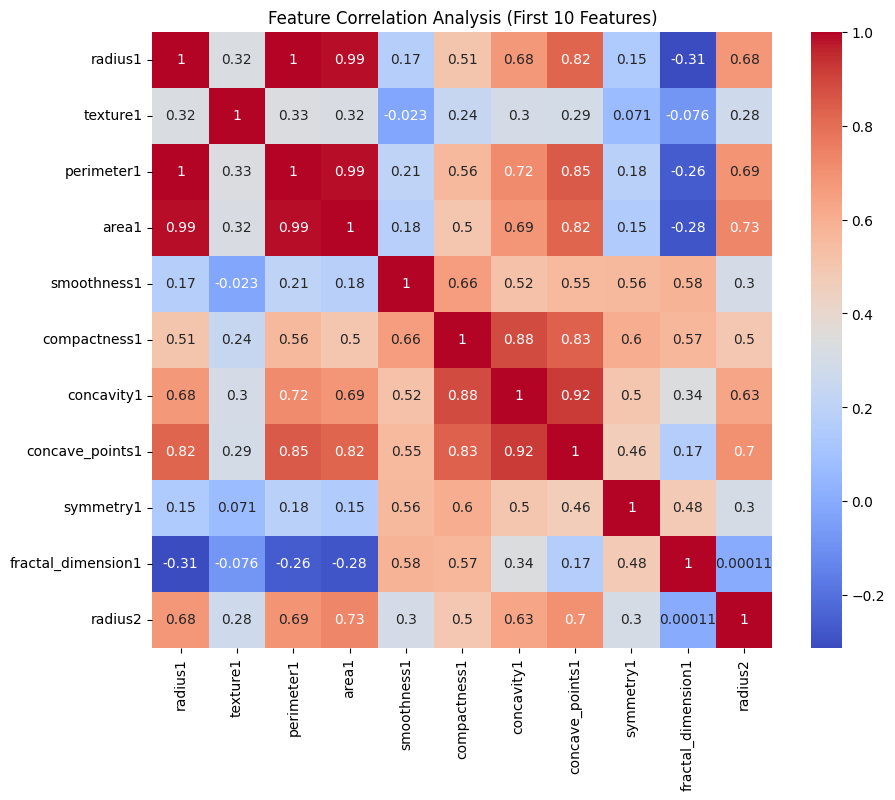
\includegraphics[width=0.65\textwidth]{corr_coeff.png}
\caption{Feature Correlation Analysis (First 10 Features)}
\end{figure}

\begin{figure}[H]
\centering
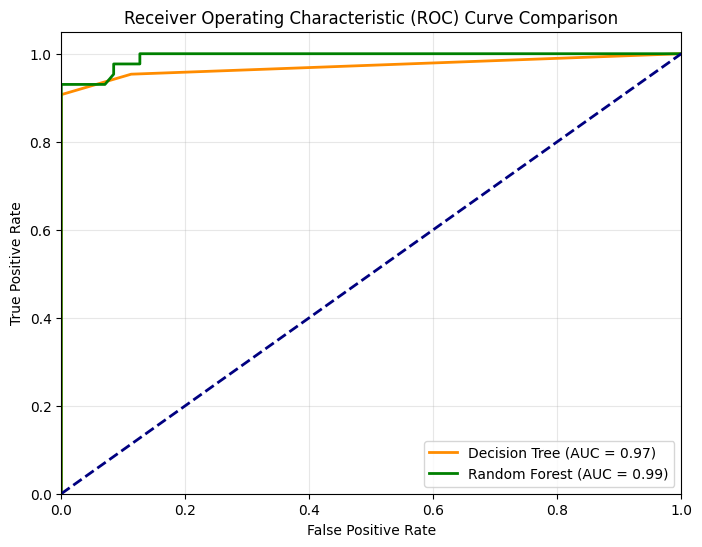
\includegraphics[width=0.75\textwidth]{roc_rf.png}
\caption{ROC Curve}
\end{figure}


%--------------------------------------------------

\section*{Observations}

\begin{itemize}
    \item \textbf{How does tree depth affect overfitting in Decision Trees?} \\
    Increasing tree depth allows the model to learn overly complex rules that perfectly classify the training data, capturing noise and outliers. This leads to high variance and severe overfitting, reducing performance on unseen test data.
    
    \item \textbf{Which hyperparameter had the greatest impact on performance?} \\
    For the Decision Tree, \texttt{max\_depth} and \texttt{min\_samples\_split} had the greatest impact by controlling tree complexity. For the Random Forest, \texttt{n\_estimators} (number of trees) significantly improved stability and reduced variance.
    
    \item \textbf{How does Random Forest improve generalization?} \\
    Random Forest improves generalization using Bootstrap Aggregation (bagging), where multiple trees are trained on different subsets of the data. Additionally, random feature selection at each split ensures the trees are less correlated. Averaging these trees reduces overall variance.
    
    \item \textbf{Did ensemble learning always improve performance? Why or why not?} \\
    Ensemble learning generally improved stability and test-set performance by reducing variance. However, if the individual trees are too weak (e.g., very shallow trees) or if the dataset is simple, the improvement over a well-tuned single tree may not be very significant.
\end{itemize}

%--------------------------------------------------

\section*{Conclusion}
Decision Tree and Random Forest models were implemented and evaluated using 5-fold cross-validation.  
Hyperparameters were selected based on average cross-validation performance, ensuring robust generalization.  
The results demonstrate that Random Forest reduces variance and improves stability compared to a single Decision Tree.

%--------------------------------------------------

\section*{References}
\begin{itemize}
    \item \href{https://scikit-learn.org/stable/modules/tree.html}{Scikit-learn: Decision Trees}
    \item \href{https://scikit-learn.org/stable/modules/ensemble.html}{Scikit-learn: Random Forest}
    \item \href{https://archive.ics.uci.edu/dataset/17/breast+cancer+wisconsin+diagnostic}{UCI Dataset}
\end{itemize}

\end{document}
